\chapter{Optimization basics}
\label{chap:optimization_basics}

\section{Optimization problems}
\label{sec:optimization_problems}

Equipped with a working knowledge of convex sets and functions, the basic
principles of optimization are now within reach. In this book, we denote an
\emph{optimization problem} by 
\index{optimization problem} 
\begin{equation}
\label{eq:optimization}
\begin{alignedat}{2}
&\minimize_x \quad && f(x) \\
&\st \quad && g_i(x) \leq 0, \; i=1,\dots,m \\ 
& && h_j(x) = 0, \; j=1,\dots,k.
\end{alignedat}
\end{equation}
Here $f$, $g_i$, $i=1,\dots,m$, and $h_j$, $j=1,\dots,k$ are functions, from 
$\R^d$ to $[-\infty,\infty]$. In problem \eqref{eq:optimization}, the
minimization is implicitly restricted to the intersection of relevant effective
domains: 
\index{effective domain}  
\[
D = \dom(f) \cap \bigcap_{i=1}^m \dom(g_i) \cap \bigcap_{j=1}^k \dom(h_j).
\]
The function $f$ in \eqref{eq:optimization} is called the \emph{criterion} or 
\emph{objective}. A \emph{feasible point} is a point in $D$ such that all
constraints (inequality and equality constraints) are met in problem
\eqref{eq:optimization}. The infimal criterion value among all feasible points
is denoted   
\index{optimization problem!criterion} 
\index{optimization problem!feasible point}     
\[
f^\star = \inf \big\{ f(x) : x \in D, \, g_i(x) \leq 0, \, i=1,\dots,m, \,
h_j(x) = 0, \, j=1,\dots,k \big\},
\]
and called the \emph{optimal value} in \eqref{eq:optimization}. A feasible point 
that achieves the optimal value is denoted $x^\star$ (note that $f^\star =
f(x^\star)$), and is called a \emph{solution} or \emph{minimizer}. 
\index{optimization problem!optimal value} 
\index{optimization problem!solution}  

It is worth being clear at the outset that a solution need not exist in an
optimization problem in general. This can happen for two distinct reasons.
First, a solution never exists in an optimization problem that is
\emph{infeasible}, which means that it has no feasible points. In this case, we
set $f^\star = \infty$ by convention. A second, more interesting case: even in
a feasible optimization problem ($f^\star < \infty$), a solution fails to
exist when the optimal value $f^\star$ is not attained. For example, informally
speaking, this happens when the criterion is minimized ``somewhere off at
infinity'' (as in $f(x) = e^{-x}$). The existence of solutions (in feasible
optimization problems) is itself a rich topic, and is covered further in Chapter 
\ref{sec:existence_minima}.       

A \emph{convex optimization problem} is one of the form
\eqref{eq:optimization} such that $f$ and $g_i$, $i=1,\dots,m$ are all
convex functions, and $h_j$, $j=1,\dots,k$ are all affine functions. In other
words, the problem 
\index{convex optimization problem}
\begin{equation}
\label{eq:convex_optimization}
\begin{alignedat}{2}
&\minimize_x \quad && f(x) \\
&\st \quad && g_i(x) \leq 0, \; i=1,\dots,m \\ 
& && Ax = b,
\end{alignedat}
\end{equation}
is convex whenever $f$ and $g_i$, $i=1,\dots,m$ are convex (and $A$ and $b$ are 
arbitrary).

In general, we will say that two optimization problems are \emph{equivalent} if 
solutions of one can be computed from solutions of the other, and vice versa. 
Clearly, problem \eqref{eq:optimization} is equivalent to:
\index{optimization problem!equivalence of problems}
\begin{alignat*}{2}
&\maximize_x \quad && -f(x) \\
&\st \quad && g_i(x) \leq 0, \; i=1,\dots,m \\ 
& && h_j(x) = 0, \; j=1,\dots,k,
\end{alignat*}
As $f$ is convex if and only if $-f$ is concave, the convex minimization 
problem \eqref{eq:convex_optimization} is hence also equivalent to a concave 
maximization problem. In this book, we will use ``optimization'' to refer to
both minimization and maximization (and we carry all definitions and notations
introduced above over to maximization problems); likewise, we will use ``convex
optimization'' to refer to both convex minimization and concave maximization.     

\begin{Remark}
In statistics, we rarely denote the parameter in an optimization problem by $x$;
we typically use $\beta$ or $\theta$ (or something else, as $x$ is usually
reserved for an input feature vector). We also rarely denote the solution to an
optimization problem by $\beta^\star$ or $\theta^\star$; we commonly use
\smash{$\hbeta$} or \smash{$\htheta$}, as these are typically seen as estimates
of population-level parameters of interest. In this book, when discussing
abstract properties of mathematical optimization, we will adhere to the standard
notation in optimization, as demonstrated above; but when discussing problems in
statistics or machine learning, we will switch fluidly to the notation more
common in these fields. This should not cause any confusion, as the meaning
(for example, what is a parameter and what is a feature) should be clear from
the context.   
\end{Remark}

\begin{Example}
The following are examples of two central optimization problems in statistics  
and machine learning. Both problems are convex. 

\begin{enumerate}[label=\alph*., ref=\alph*]
\item Given responses $y_i \in \R$ and associated feature vectors $x_i \in
  \R^d$, for $i=1,\dots,n$, the \emph{least absolute selection and shrinkage
    operator (lasso)} is a sparse estimator of the coefficients $\beta$ in a
  linear model (to $y_i$ predict from $x_i^\T \beta$), defined by the
  optimization problem: 
  \index{lasso}
  \begin{equation}
  \label{eq:lasso_sum}
  \minimize_\beta \quad \frac{1}{2} \sum_{i=1}^n (y_i - x_i^\T \beta)^2 +  
  \lambda \sum_{j=1}^d |\beta_j|.
  \end{equation}
  Here $\lambda \geq 0$ is a tuning parameter governing the tradeoff between 
  goodness-of-fit (first term) and sparsity (second term). The above also has a
  more compact form, denoting by $y \in \R^n$ the response vector and $X \in
  \R^{n \times d}$ the feature matrix (whose $i\th$ row is $x_i^\T$):  
  \begin{equation}
  \label{eq:lasso}
  \minimize_\beta \quad \frac{1}{2} \|y - X \beta\|_2^2 + \lambda \|\beta\|_1. 
  \end{equation}
  For insight into the sparsity-inducing property of $\ell_1$ penalties, from
  the perspective of proximal mappings, see Chapter
  \ref{sec:proximal_optimality}.    

  \noindent
  Note: by default, we will always omit an intercept term in the lasso
  regression model as it can be accounted for by centering $y$ and each column
  of $X$, before solving \eqref{eq:lasso}; see Example \parref{xa:lasso_partial}
  for a generalization.   

\item Given class labels $y_i \in \{ -1, 1\}$ and feature vectors $x_i \in
  \R^d$, for $i=1,\dots,n$, the \emph{support vector machine (SVM)} is a
  large-margin linear classifier (to predict $y_i$ from the sign of $\beta_0
  + x_i^\T \beta$), defined by the optimization problem:   
  \index{support vector machine} 
  \begin{equation}
  \label{eq:svm}
  \begin{alignedat}{2}
  &\minimize_{\beta_0,\beta,\xi} \quad
  && \frac{1}{2} \|\beta\|_2^2 + C \sum_{i=1}^n \xi_i \\ 
  &\st \quad && y_i (\beta_0 + x_i^\T \beta) \geq 1-\xi_i, \;  i=1,\dots,n \\
  & && \xi \geq 0.
  \end{alignedat}
  \end{equation}
  Here $C \geq 0$ is a tuning parameter governing the tradeoff between the size
  of the margin (the first term above is actually the \emph{inverse} margin; see
  Exercise \ref{ex:svm_margin}) and violations to the margin condition (the
  second term is the sum of violation costs, and each violation is an instance  
  of a prediction $\beta_0 + x_i^\T \beta$ lying on the wrong side of the
  margin).               
\end{enumerate}
\end{Example}

It is helpful to introduce some additional notation for an optimization problem 
\eqref{eq:optimization} in which the criterion is identically zero $f(x)=0$ (or, 
equal to any finite constant). We call this a \emph{feasbility problem}. A
feasibility problem effectively seeks whether the constraints can be satisfied,
and if so, seeks any point $x^\star$ that is feasible. We write it as  
\index{feasibility problem} 
\begin{equation}
\label{eq:feasibility}
\begin{alignedat}{2}
&\find \quad && x \\
&\st \quad && g_i(x) \leq 0, \; i=1,\dots,m \\ 
& && h_j(x) = 0, \; j=1,\dots,k.
\end{alignedat}
\end{equation}
A \emph{convex feasibility problem} is one in which the constraint functions
satisfy the usual requirements: $g_i$, $i=1,\dots,m$ are convex and $h_j$,
$j=1,\dots,k$ are affine.   

\section{Properties of convex problems} 
\label{sec:properties_convex_problems}

Next we describe several important properies of convex optimization problems,
beginning with the most important one.

\paragraph{Local solutions are global solutions.} 
\parlab{par:convex_local}

A point \smash{$\bar{x}$} is called a \emph{local solution} of the problem
\eqref{eq:optimization} if it is feasible and there is some $\delta>0$ such that 
\index{optimization problem!local solution}  
\[
f(\bar{x}) \leq f(x), \quad \text{for all feasible $x$ such that
$\|x - \bar{x}\|_2 \leq \delta$}.
\]
For a convex optimization problem, the following holds: any local solution
\smash{$\bar{x}$} must also be a global solution, in that \smash{$f(\bar{x})
  \leq f(x)$} for all feasible points $x$. (This is also simply called a
solution, and we add the modifier ``global'' here to emphasize the difference to
the local condition.) This result is so important that it may as well be called
the \emph{fundamental theorem of convex optimization}. 

The proof of this fundamental result is elementary. It can be broken into two  
steps. The first step is to check that for the convex problem
\eqref{eq:convex_optimization}, the set of feasible points is a convex set,
which follows from convexity of the set $D$, convexity of the functions $f$ and
$g_i$, $i=1,\dots,m$, and the linear structure of the equality constraints 
$Ax=b$ (Exercise \ref{ex:convex_solution} part a).  

The second step proceeds by contradiction. If \smash{$\bar{x}$} is not a global
solution, then there is a feasible point $y$ such that \smash{$f(y) <
  f(\bar{x})$}. Since \smash{$\bar{x}$} is locally optimal, we must have
\smash{$\|y - \bar{x}\|_2 > \delta$}. However, we can choose some $t \in (0,1)$ 
such that \smash{$x = ty + (1-t) \bar{x}$} satisfies \smash{$\|x - \bar{x}\|_2
  \leq \delta$} (for example, take \smash{$t = \delta / \|y - \bar{x}\|_2$}).
By convexity of the feasible set, we know that $x$ is feasible. By convexity of
$f$,  
\[
f(x) \leq t f(y) + (1-t) f(\bar{x}) < f(\bar{x}),
\]
where the last inequality is strict since \smash{$f(y) < f(\bar{x})$} and
$t>0$. The above display is a contradiction of local optimality, which proves
that such a $y$ cannot exist, and \smash{$\bar{x}$} must be globally optimal. 

\paragraph{Solution sets are convex.} 
\parlab{par:convex_solution} 

A related property of a convex optimization problem is that its solution set,
which we can denote by 
\[
S^\star = \{ x^\star: \text{$x^\star$ is a solution in
  problem \eqref{eq:convex_optimization}} \},
\]
is itself a convex set. The proof is similar to the proof that the feasible set
of a convex problem is convex (Exercise \ref{ex:convex_solution} part b).
Convexity of $S^\star$ has the following interesting implication: a convex
problem can have 0, 1, or infinitely many solutions---no other number is
possible!  

An important refinement is possible when the criterion $f$ in a convex problem
is strictly convex. In this case, the solution set $S^\star$---if
nonempty---must be a singleton (Exercise \ref{ex:convex_solution} part d).
% In other words, for a convex optimization problem with strictly convex
% criterion, if a solution exists, then it must be unique.  
\index{convex optimization problem!uniqueness of solution}

\paragraph{First-order optimality condition.}
\parlab{par:first_order_optimality}   

Denote by 
\[
C = \{ x \in D : g_i(x) \leq 0, \, i=1,\dots,m, \, Ax = b \}
\]
the feasible set of the convex optimization problem
\eqref{eq:convex_optimization}. For a differentiable criterion $f$, a point $x
\in C$ is a solution if and only if 
\index{first-order optimality condition} 
\begin{equation}
\label{eq:first_order_optimality}
\nabla f(x)^\T (y - x) \geq 0, \quad \text{for all $y \in C$}.
\end{equation}
This is called the \emph{first-order optimality condition} for problem
\eqref{eq:convex_optimization}. It can be interpreted as follows: any move from 
$x$ in the direction of another feasible point cannot decrease the criterion
$f$, according to the first-order Taylor expansion of $f$ at $x$. In the
unconstrained case (which means $m=r=0$, so there are no constraints), the
feasible set is $C=\dom(f)$, and since a differentiable function has an open
effective domain (by assumption, see Appendix \ref{sec:derivative}), the
first-order optimality condition \eqref{eq:first_order_optimality} reduces to
the more familiar zero-gradient condition    
\begin{equation}
\label{eq:zero_gradient}
\nabla f(x) = 0.
\end{equation}
To see this observe that for sufficiently small $\delta>0$, we have $y = x +
\delta v \in \dom(f)$ for any $v$, which from  \eqref{eq:first_order_optimality}
will lead us to the conclusion that $\nabla f(x)^\T v = 0$ for any $v$, implying
\eqref{eq:zero_gradient}.  

We note that the first-order optimality condition
\eqref{eq:first_order_optimality} is actually a special case of what we will
call the subgradient optimality condition, to be encountered later in Chapter  
\ref{sec:subgradient_optimality}. 

\begin{Example}
The following are three examples of the first-order optimality condition for
convex optimization. 

\begin{enumerate}[label=\alph*., ref=\alph*]
\item For a differentiable convex optimization problem with only equality
  constraints, 
  \[
  \minimize_x \quad f(x) \quad \st \quad Ax = b,
  \]
  the first-order optimality condition \eqref{eq:first_order_optimality} reduces
  to  
  \index{Lagrange multiplier condition} 
  \begin{equation}
  \label{eq:lagrange_multiplier}
  \nabla f(x) + A^\T v = 0, \quad \text{for some $v$}.
  \end{equation}
  The argument justifying \eqref{eq:lagrange_multiplier} is similar to that used
  in the unconstrained case to justify \eqref{eq:zero_gradient} (see Exercise
  \ref{ex:lagrange_multiplier}). The condition \eqref{eq:lagrange_multiplier}
  is known as a \emph{Lagrange multiplier condition}, and it will be generalized
  by the Karush-Kuhn-Tucker conditions, which we will study later in Chapter 
  \ref{chap:kkt_conditions}. 

\item The Euclidean projection operator $P_C$ onto a convex set $C \subseteq 
  \R^d$ can be formulated in terms of differentiable convex optimization. In 
  particular, for any $x \in \R^d$, its projection $P_C(x)$ onto $C$ is the
  unique solution of the optimization problem  
  \index{projection}
  \[
  \minimize_z \quad \|x - z\|_2^2 \quad \st \quad z \in C.
  \]
  The condition \eqref{eq:first_order_optimality} (now interpreted with respect
  to $z$) gives, after rearrangement,  
  \index{projection!variational inequality} 
  \begin{equation}
  \label{eq:variational_inequality}
  (x - z)^\T (z - y) \geq 0, \quad \text{for any $y \in C$}. 
  \end{equation}
  This is often referred to as the \emph{variational inequality} for a
  projection. It says that the vector pointing from $z$ to $x$ must have a
  positive inner product with the vector pointing from $y$ to $z$, for any $y
  \in C$. See Figure \ref{fig:variational_inequality}.    

\item \parlab{xa:zero_gradient_quadratic}
  For a convex quadratic function \smash{$f(x) = \frac{1}{2} x^\T A x + b^\T x
    + c$} (where $A \succeq 0$) the first-order optimality condition
  \eqref{eq:zero_gradient} says that $x$ minimizes $f$ if and only if
  \begin{equation} 
  \label{eq:zero_gradient_quadratic}
  Ax + b =  0
  \end{equation}
  We can now reason in cases. 
 \begin{enumerate}[label=(\roman*)]
 \item If $A$ is invertible, then the only solution to
   \eqref{eq:zero_gradient_quadratic} is $x^\star = -A^{-1} b$. 

\item If $A$ is singular and $b \in \col(A)$, then there are infinitely many
  solutions to \eqref{eq:zero_gradient_quadratic}, of the form $x^\star = x_0 +
  v$ where $x_0$ is one particular solution ($Ax_0 + b = 0$) and $v$ is any
  element in $\nul(A)$, the null space of $A$. 

 \item If $A$ is singular and $b \notin \col(A)$, then
   \eqref{eq:zero_gradient_quadratic} has no solution, which means that $f$ does
   not have a minimizer (it does not attain its infimum). An example in which
   this occurs is the 2-dimensional convex quadratic $f(x) = x_1^2 - x_2$. 
 \end{enumerate}
\end{enumerate}
\end{Example}

\begin{figure}[tb]
\centering
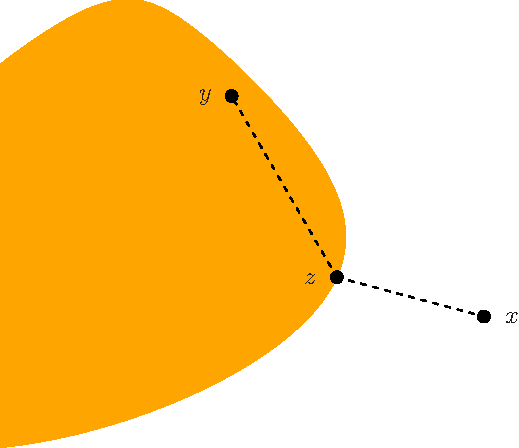
\includegraphics[width=0.475\textwidth]{fig/variational_inequality.pdf}
\caption{Illustration of the variational inequality that determines the
  optimality of the projection $z$ of a point $x$ onto a convex set. The angle
  between the line segments $zx$ and $zy$ must be at least a right angle (at
  least $90^\circ$), for any other point $y$ in the set.} 
\label{fig:variational_inequality}
\end{figure}

\section{Problem transformations}

We walk through various general transformations of optimization problems that
can make a problem easier to solve or easier to understand. In each case, we do
not assume convexity outright, but we do highlight the situations in which more
can be said about convex optimization.

\paragraph{Characteristic formulation.} 

Denote the feasible set of the optimization problem \eqref{eq:optimization} by  
\[
C = \{ x \in D : g_i(x) \leq 0, \, i=1,\dots,m, \, h_j(x) = 0, \, j=1,\dots,k
\} 
\]
Then \eqref{eq:optimization} is equivalent to the unconstrained optimization
problem 
\index{optimization problem!characteristic form}
\begin{equation}
\label{eq:characteristic_formulation}
\minimize_x \quad f(x) + I_C(x),
\end{equation}
where $I_C$ is the characteristic function of $C$, defined in
\eqref{eq:characteristic_function}. For convex optimization, recall that the
criterion $f$ and feasible set $C$ must both be convex, which implies 
$f + I_C$ is also convex. In others words, problem
\eqref{eq:characteristic_formulation} is convex provided that the original
problem \eqref{eq:optimization} is. 

We refer to \eqref{eq:characteristic_formulation} as the \emph{characteristic
  formulation} of problem \eqref{eq:optimization}. Though the characteristic 
formulation is not (typically) more practically convenient than the original
problem, it can still lead to useful insights. For example, in the convex case
(with $f$ and $C$ convex), applying the subgradient optimality condition to
\eqref{eq:characteristic_formulation} yields a natural generalization of the
first-order optimality condition in \eqref{eq:first_order_optimality}. This
will be covered in Chapter \ref{sec:subgradient_optimality}.

\paragraph{Partial optimization.} 
\parlab{par:partial_optimization}

For any function $g$, it holds that (Exercise \ref{ex:inf_sup_rules} part a):
\[
\inf_{x_1, x_2} \, g(x_1, x_2) = \inf_{x_1} \, G(x_1), 
\]
where $G(x_1) = \inf_{x_2} g(x_1,x_2)$. If we work from the characteristic
formulation \eqref{eq:characteristic_formulation}, for a general optimization
problem, and we treat $x$ as a block variable $x=(x_1,x_2)$, then we can apply
the above result to $g = f + I_C$: this tells us that we can perform
partial optimization---namely, optimization over $x_2$---to produce an
equivalent optimization problem, in $x_1$ alone. 

This statement can be made more concrete in the case that, for each fixed $x_1$,
the infimum of $g(x_1,x_2)$ over $x_2$ is attained, and we denote a
minimizer by $x^\star_2(x_1)$. Then $G(x_1) = g(x_1, x^\star_2(x_1))$, and 
\[
\minimize_{x_1,x_2} \quad f(x_1, x_2) \quad \st \quad (x_1,x_2) \in C, 
\]
is equivalent to 
\index{partial optimization}
\[
\minimize_{x_1} \quad F(x_1) \quad \st \quad x_1 \in \tilde{C},
\]
with \smash{$F(x_1) = \inf_{x_2 : (x_1,x_2) \in C} f(x_1,x_2) = f(x_1,
  x^\star_2(x_1))$}, and \smash{$\tilde{C} = \{x_1 : \text{$(x_1, x^\star_2  
    (x_1)) \in C$} \}$}. It is worth noting that the setting of convex
optimization, where $f$ and $C$ are convex in the former problem (second-to-last  
display), we know by Property \parref{par:function_infimum} that the latter
problem (last display) is also convex, provided that $F$ is nowhere equal to
$-\infty$.  

\begin{Example}
The following are two examples of partial optimization in convex problems. 

\begin{enumerate}[label=\alph*., ref=\alph*]
\item \parlab{xa:lasso_partial}
  For a response $y \in \R^n$, and features $X_1 \in \R^{n \times  d_1}$ and 
  $X_2 \in \R^{n \times   d_2}$, consider 
  \[
  \minimize_{\beta_1, \beta_2} \quad \frac{1}{2} \|y - X_1\beta_1 -
  X_2\beta_2\|_2^2 + \lambda \|\beta_1\|_1. 
  \]
  This is like the (usual form) lasso problem \eqref{eq:lasso}, but where the
  $\beta_2$ block of coefficients is not penalized. Since the above problem is
  simply a quadratic in $\beta_2$, we can minimize over it, for fixed $\beta_1$,
  and find that a minimizer \smash{$\hbeta_2(\beta_1)$} (which is unique if and
  only if $X_2$ is full column rank) satisfies       
  \[
  X_2 \hbeta_2(\beta_1) = P_{X_2} (y - X_1\beta_1)
  \]
  where \smash{$P_{X_2} = X_2 (X_2^\T X_2)^\pinv X_2$} is the projection onto
  $\col(X_2)$. By plugging this into the above original problem, we get an
  equivalent problem     
  \[
  \minimize_{\beta_1} \quad \frac{1}{2} \|P_{X_2}^\perp y - P_{X_2}^\perp
  X_1\beta_1\|_2^2+ \lambda \|\beta_1\|_1,  
  \]
  where \smash{$P_{X_2}^\perp = I - P_{X_2}$} is the projection onto the
  orthocomplement $\col(X_2)$. Note that this is a (usual form) lasso problem
  with response \smash{$P_{X_2}^\perp y$} and feature matrix
  \smash{$P_{X_2}^\perp  X_1$}.   

\item Consider the SVM problem \eqref{eq:svm}. Note that, after rearrangement,
  the linear constraints are equivalent to
  \[
  \xi_i \geq \big[1 - y_i(\beta_0 + x_i^\T \beta_0)\big]_+, \quad i=1,\dots,n, 
  \]
  where $a_+ = \max\{a,0\}$ denotes the positive part of $a$. Looking at the
  criterion in \eqref{eq:svm}, we can see that a minimizer over the $\xi$ block
  of variables, as a function of the others, achieves all equalities in the
  above set of inequalities (and this is unique if $C>0$): 
  \[
  \hat\xi_i(\beta_0,\beta) = \big[1 - y_i(\beta_0 + x_i^\T \beta_0)\big]_+,
  \quad i=1,\dots,n.
  \]
  This holds as increasing $\xi_i$ from \smash{$\hat\xi_i(\beta_0,\beta)$} by 
  any amount $\delta \geq 0$ increases the criterion by $C \delta \geq 0$.
  Plugging this in results in what is called the \emph{hinge form} of the SVM 
  problem: 
  \index{support vector machine!hinge form}
  \begin{equation}
  \label{eq:svm_hinge}
  \minimize_{\beta_0,\beta} \quad C \sum_{i=1}^n \big[1 - y_i(\beta_0 + x_i^\T 
  \beta_0)\big]_+ + \frac{1}{2} \|\beta\|_2^2.
  \end{equation}
  This has a familiar ``loss + penalty'' form, much like ridge regression, but
  with the hinge loss replacing what would be the squared loss in the ridge 
  regression problem. 
\end{enumerate}
\end{Example}

\paragraph{Monotone criterion transformation.} 
\parlab{par:monotone_transformation}

If $\phi$ is increasing then problem \eqref{eq:optimization}, with feasible set
abbreviated by $C$, is equivalent to 
\index{optimization problem!criterion transformation}
\[
\minimize_x \quad \phi(f(x)) \quad \st \quad x \in C,
\]
and hence also equivalent to, for any decreasing $\psi$,
\[
\maximize_x \quad \psi(f(x)) \quad \st \quad x \in C.
\]
It is worth noting that monotone transformations can influence convexity or
concavity in nontrivial ways. For example, \smash{$f(x) = e^{-x^2}$} is neither
convex nor concave, but for $\psi(u) = -\log(u)$ (decreasing) we get $\psi(f(x))
= x^2$, which is convex. Therefore it can be useful to apply a monotone
transformation to the criterion in an optimization problem, because it can turn
a nonconvex problem into a convex problem. An important example of this is
maximum likelihood estimation in log-concave families, as discussed in Chapter 
\ref{sec:maximum_likelihood}. 

It is also worth noting that monotone transformations can just as well be
applied in order to recast constraints; for example, if $\phi$ is increasing and
$\psi$ decreasing, then 
\[
g(x) \leq 0 \iff \phi(g(x)) \leq \phi(0) \iff \psi(g(x)) \geq \psi(0).
\]

\paragraph{One-to-one variable transformation.} 

If $\phi : \R^k \to \R^d$ is one-to-one (meaning, $u \not= v \implies \phi(u)
\not= \phi(v)$), and $\ran(\phi)$ contains the feasible set $C$ in problem
\eqref{eq:optimization}, then \eqref{eq:optimization} is equivalent to   
\index{optimization problem!variable transformation}
\[
\minimize_y \quad f(\phi(y)) \quad \st \quad \phi(y) \in C. 
\]
Such a variable transformation can be useful for various reasons: for example,
it can be dimension-reducing ($k < d$), or it can transform a nonconvex problem
into a convex one.  

\begin{Example}
An optimization problem with linear equality constraints,
\begin{alignat*}{2}
&\minimize_x \quad && f(x) \\
&\st \quad && g_i(x) \leq 0, \; i=1,\dots,m \\ 
& && Ax = b, 
\end{alignat*}
can always be recast, via variable transformation, into one that has only
inequality constraints. Assuming $Ax = b$ has a solution $x_0$ (otherwise the
above problem is infeasible), we can write any and all solutions as $x = x_0 +
Vy$, where the columns of $V \in \R^{d \times k}$ form a basis for $\nul(A)$ and  
$y \in \R^k$. Therefore the above problem is equivalent to 
\begin{alignat*}{2}
&\minimize_y \quad && f(x_0+Vy) \\
&\st \quad && g_i(x_0+Vy) \leq 0, \; i=1,\dots,m.
\end{alignat*}
Though the above two problems are always equivalent, it is not always a good
idea, practically speaking, to seek to solve the second instead of the
first---and this is not a simple matter of comparing $k$ to $d$. Eliminating
equality constraints can alter problem structure in nontrivial ways. For
example, if $A$ sparse, then it might not be easy (or even possible) to find a
sparse basis $V$ for $\nul(A)$, and such sparsity could be lost in moving
from the first problem to the second. This could make a big difference in
practice, depending on the specifics (the size of the problem, the algorithm 
one has in mind for computing a solution, etc.).
\end{Example}

\paragraph{Slack variables.} 

Proceeding in somewhat of an opposite direction to the last example (eliminating
equality constraints), we can replace all inequality constraints in
\eqref{eq:optimization} with equality constraints, using the following
equivalent formulation: 
\begin{alignat*}{2}
&\minimize_{x,s} \quad && f(x) \\
&\st \quad && g_i(x) + s_i = 0, \; i=1,\dots,m \\ 
& && h_j(x) = 0, \; j=1,\dots,k, \\
& && s \geq 0.
\end{alignat*}
The variables $s_i$, $i=1,\dots,m$ here are called \emph{slack variables}. 
Comparing the above problem to \eqref{eq:optimization}, we have increased the
problem dimension (from $d$ to $d+m$); however, in some settings, reducing the
inequality constraints to simple nonnegativity constraints brings other
advantages.
\index{slack variable}

In general, introducing slack variables can turn a convex problem into a
nonconvex one; only for an affine function $g_i$ is the equality constraint
$g_i(x) + s_i = 0$ affine in $x,s$.       

\paragraph{Relaxation.} 

If \smash{$\tilde{C} \supseteq C$}, then 
\index{relaxation}
\[
\minimize_x \quad f(x) \quad \st \quad x \in \tilde{C}
\]
is called a \emph{relaxation} of 
\[
\minimize_x \quad f(x) \quad \st \quad x \in C.
\]
The following properties are easily verified: 
\begin{enumerate}[label=(\roman*)]
\item if \smash{$f^\star(C), f^\star(\tilde{C}), $} denote the optimal values in 
  the original and relaxed problems, respectively, then it always holds that 
  \smash{$f^\star(\tilde{C}) \leq f^\star(C)$};  
\item if $x^\star$ denotes a solution in the relaxed problem and $x^\star \in
  C$, then $x^\star$ is also a solution in the original problem and
  \smash{$f^\star(\tilde{C}) = f^\star(C)$}. 
\end{enumerate}
If \smash{$f^\star(\tilde{C}) = f^\star(C)$}, then the relaxation is said to be 
\emph{tight}. If the relaxation is a convex optimization problem, then it is
called a \emph{convex relaxation}. 
\index{convex relaxation}

% We note that a more general notion of relaxation can be obtained by replacing    
% the criterion in the first problem above by a function \smash{$\tilde{f}$}
% with \smash{$\tilde{f} \leq f$}. In such a case, property (i) continues to
% hold.    

\begin{Example}
\label{xa:best_rank_approximation}
Consider the problem of finding the best rank $k$ approximation of $X \in \R^{n
  \times d}$, for a given positive integer $k \leq \rank(X)$,   
\begin{equation}
\label{eq:best_rank_approximation}
\minimize_\Theta \quad \|X - \Theta\|_F^2 \quad \st \quad \rank(\Theta) = k,
\end{equation}
where the Frobenius norm of a matrix $A \in \R^{n \times d}$ is denoted
\smash{$\|A\|_F = \sqrt{\sum_{i=1}^n \sum_{j=1}^d A^2_{ij}}$}. The above problem
is nonconvex because of its constraint ($\rank(\cdot)$ is not an affine function
over matrices; it is not even a convex function). Nevertheless, it has a
well-known solution, by the \emph{Eckart-Young-Mirsky theorem}, in terms of the
singular value decomposition (SVD) of $X$:   
\index{Frobenius norm}
\index{Eckart-Young-Mirsky theorem} 
\index{principal components analysis} 
\begin{equation}
\label{eq:best_rank_solution}
\hat\Theta = \sum_{i=1}^k \sigma_i u_i v_i^\T.
\end{equation}
Here $\sigma_i$ denotes the $i\th$ largest singular value of $X$, and $u_i \in 
\R^n, v_i \in \R^d$ are the corresponding left and right singular vectors of
$X$. The solution in \eqref{eq:best_rank_solution} is unique if and only if 
$\sigma_k \not= \sigma_{k+1}$. In statistics---where $X$ would typically
represent a data matrix ($n$ samples observed over $d$ features)---we  
call \smash{$\hat\Theta$} the reconstruction of $X$ from its top $k$
\emph{principal components}.

\setlength{\parindent}{\normalparindent}
As it turns out, the nonconvex problem \eqref{eq:best_rank_approximation} 
admits, after reformulation, a tight convex relaxation. To see this, we start
by reformulating the problem as (Exercise \ref{ex:best_rank_approximation} part
a):  
\begin{equation}
\label{eq:best_projection_min}
\minimize_P \quad \|X - XP\|_F^2 \quad \st \quad P \in \cP_k,
\end{equation}
where $\cP_k$ denotes the set of rank $k$ projection matrices, from $\R^d$ to 
$\R^d$. (A solution here is given by \smash{$\hat{P} = \sum_{i=1}^k v_i
  v_i^\T$}, which is again unique iff $\sigma_k \not= \sigma_{k+1}$.)  Now    
define an inner product on matrices $A,B \in \R^{n \times d}$ by $\langle A,
B \rangle = \tr(A^\T B)$, and observe that $\|A\|_F^2 = \langle A, A \rangle$. 
%Expanding the criterion in \eqref{eq:best_projection_min}, dropping terms
%that do not depend on $P$, and applying properties of projection matrices,
After some basic manipulations (Exercise \ref{ex:best_rank_approximation} part  
b), we arrive at the equivalent problem
\begin{equation}
\label{eq:best_projection_max}
\maximize_P \quad \langle S, P \rangle \quad \st \quad P \in \cP_k,
\end{equation}
where $S = X^\T X$. A convex relaxation of \eqref{eq:best_projection_max} is
thus given by
\index{convex relaxation}
\begin{equation}
\label{eq:fantope_projection}
\maximize_P \quad \langle S, P \rangle \quad \st \quad P \in \cF_k,
\end{equation}
where $\cF_k = \conv(\cP_k)$. Furthermore, the relaxation
\eqref{eq:fantope_projection} is tight, which follows by arguing that the
maximum of the linear criterion in \eqref{eq:fantope_projection} is attained by 
one of the extreme points of $\cF_k$, which are exactly the rank $k$ projection
matrices in $\cP_k$ (Exercise \ref{ex:best_rank_approximation} part c).

It is interesting to note that the set $\cF_k = \conv(\cP_k)$, the convex hull
of rank $k$ projection matrices, can be written explicitly as (Exercise
\ref{ex:best_rank_approximation} part d):    
\begin{equation}
\label{eq:fantope}
\cF_k = \{ P \in \SS^d : 0 \preceq P \preceq I, \, \tr(P) = k \}.
\end{equation}
This is often referred to as the \emph{Fantope} of order $k$, named after
mathematician Ky Fan.
\index{Fantope}
\end{Example}

\section{Existence of minima*}
\label{sec:existence_minima}
\index{optimization problem!existence of solution}

It is not hard to see that some notion of continuity is required in order to
guarantee the existence of minima (guarantee a function attains its infimum) in
general. For example, the function
\begin{equation}
\label{eq:discontinuous_quadratic}
f(x) = \begin{cases}
x^2 & \text{if $x \not= 0$} \\
1 & \text{if $x = 0$}
\end{cases}
\end{equation}
has an infimum of 0, but no minimizer. In order to prevent such behavior, we
need some condition that restricts what can happen as we move along a sequence
that drives a function to its infimum.  

A weak notion of continuity that is useful for reasoning about the existence  
of minima is called \emph{lower semicontinuity}. A function $f : \R^d \to 
[-\infty, \infty]$ is lower semicontinuous at a point $x$ if, for any sequence 
such that \smash{$\lim_{k \to \infty} x_k = x$}, it holds that 
\[
f(x) \leq \liminf_{k \to \infty} f(x_k). 
\]
(We emphasize that in our definition the point $x$ does not need to be in
$\dom(f)$, and the sequence \smash{$\{x_k\}_{k=1}^\infty$} does need to be
contained in $\dom(f)$.)  We call a function $f$ lower semicontinuous if it
is lower semicontinuous at each $x \in \R^d$. The next lemma collects a few 
relevant equivalences.

\index{sublevel set}
\begin{Lemma}
\label{lem:lower_semicontinuous}
For any $f : \R^d \to [-\infty, \infty]$, the following statements are equivalent:
\begin{enumerate}[label=(\roman*)]
\item $f$ is lower semicontinuous;
\item its sublevel sets $\{x : f(x) \leq t\}$, $t \in \R$ are all closed;
\item its epigraph $\epi(f) = \{(x,t) : f(x) \leq t\}$ is closed. 
\end{enumerate}
\end{Lemma}

\index{closed function}
We call a function \emph{closed} if its epigraph is closed, and we use this
terminology interchangeably with lower semicontinuity (since, according to the
above, they are equivalent properties). Recall by Theorem
\ref{thm:smoothness_properties} part (i) that a convex function $f$ is
necessarily continuous, thus lower semicontinuous, at each $x \in
\interior(\dom(f))$; in this light, we can see that a for convex function,
closedness is really just a matter of its behavior on the boundary (if nonempty)
of its effective domain.

Lower semicontinuity does rule out examples such as
\eqref{eq:discontinuous_quadratic}, but cannot by itself guarantee the existence
of minima. For example, consider $f(x) = e^{-x}$. Hence, it seems that in order
to guarantee a function $f$ attains its infimum, we should pair lower
semicontinuity with a condition that rules out the possibility of $f$ being
minimized ``somewhere off at infinity''.

First, we recount (a generalization of) \emph{Weierstrass' theorem}, which
applies broadly to a function with compact sublevel sets. Here, and in the rest
of the results in this section, we implicitly assume that $f \not= \infty$, that
is, $\dom(f) \not= \emptyset$, to rule out a trivial case in which $f$ does not 
attain its infimum.   

\index{Weierstrass' theorem}
\begin{Theorem}[Weierstrass' theorem]
\label{thm:weierstrass}
A closed function $f : \R^d \to (-\infty, \infty]$ has a nonempty and compact
set of minima if there exists some $t \in \R$ such that $\{ x : f(x) \leq t\}$
is nonempty and bounded. Two simple sufficient conditions for the latter to
hold (existence of a nonempty bounded sublevel set) are:
\begin{enumerate}[label=(\roman*)]
\item $\dom(f)$ is bounded; 
\item $f$ is \emph{coercive}, which means that \smash{$\lim_{k \to \infty}
    f(x_k) \to \infty$} whenever \smash{$\lim_{k \to \infty} \|x_k\|_2 \to
    \infty$}.  
  \index{coercive function}  
\end{enumerate}
\end{Theorem}

% For example, Proposition 3.2.1 in Bertsekas (2009)

The role of closedness of $f$ in Theorem \ref{thm:weierstrass} is to ensure
closedness of its sublevel sets; combined with the assumption that $\{x : f(x)
\leq t\}$ is nonempty and bounded, for some $t \in \R$, we see that such a
sublevel is indeed compact. Hence the sublevel sets of $f$ at all levels $s \leq 
t$ are also compact. The result follows by recognizing that the set of minima
of $f$ is the intersection of its nonempty sublevel sets; see Exercise
\ref{ex:weierstrass}.

In the constrained case, for minimization of $f$ over a set $C \subseteq
\dom(f)$, the following is a special case of the Weierstrass theorem, obtained
by applying Theorem \ref{thm:weierstrass} to $f + I_C$.
% (and placing simple conditions on $f,C$ in order for $f + I_C$ to meet the 
% conditions in the theorem).  

\begin{Corollary}
For a function $f : \R^d \to (-\infty, \infty]$, lower semicontinuous at every
point in a nonempty closed set $C \subseteq \dom(f)$, the optimization problem    
\[
\minimize_x \quad f(x) \quad \st \quad x \in C
\]
has a nonempty and compact solution set if there exists $t \in \R$ such that
$\{x \in C : f(x) \leq t\}$ is nonempty and bounded. Two simple sufficient
conditions for the latter to hold are:
\begin{enumerate}[label=(\roman*)]
\item $C$ is bounded; 
\item $f$ is \emph{coercive on $C$}, which means that \smash{$\lim_{k \to
      \infty} f(x_k) \to \infty$} whenever \smash{$\{x_k\}_{k=1}^\infty
    \subseteq C$} and \smash{$\lim_{k \to   \infty} \|x_k\|_2 \to \infty$}. 
\end{enumerate}
\end{Corollary}

For a convex function, more can be said. Towards this end, it is helpful to
introduce the notion of a \emph{direction of recession} of a convex function
$f$: this is a direction $v \in \R^d$ such that 
\index{direction of recession} 
\begin{equation}
\label{eq:direction_recession}
\text{$\lambda \mapsto f(x + \lambda v)$ is a nonincreasing function of 
  $\lambda \in \R$}, \quad \text{for all $x \in \dom(f)$}.  
\end{equation}
Viewed geometrically, this is a statement about the existence of rays (running
parallel to $v$) within the sublevel sets of $f$. The next lemma provides the 
details. It helps to analogously define a \emph{direction of recession} of a
convex set $C \subseteq \R^d$: this is $v \in \R^d$ such that $\{x + \lambda v :
\lambda \geq 0\} \subseteq C$, for all $x \in C$.  

\begin{Lemma}
\label{lem:direction_recession}
For a closed convex function $f$, the following are equivalent: 
\begin{enumerate}[label=(\roman*)]
\item $v$ is a direction of recession of $f$;
% \item \smash{$\liminf_{\lambda \to \infty} f(x + \lambda v) < \infty$} for all
%   $x \in \dom(f)$; 
% \item \smash{$\liminf_{\lambda \to \infty} f(x + \lambda v) < \infty$} for one
%   $x \in \dom(f)$;
\item $v$ is a direction of recession of every $V_t = \{x : f(x) \leq t\}$, $t
  \in \R$; 
\item there exists $t \in \R$ and $x \in V_t$ such that $\{x + \lambda v :
  \lambda \geq 0\} \subseteq V_t$;  
\item there exists $x \in \dom(f)$ such that $\lambda \mapsto f(x + \lambda v)$ 
  is nonincreasing.
\end{enumerate}

\index{sublevel set}
Furthermore, as for the other direction, the following are equivalent: 
\begin{enumerate}[resume, label=(\roman*)]
\item $f$ has no directions of recession; 
\item no sublevel set of $f$ contains a ray;
\item every sublevel set of $f$ is bounded. 
\end{enumerate}
\end{Lemma}

The key fact underlying the above lemma is that, for a closed convex set $C$:  
\begin{equation}
\label{eq:one_iff_all}
\{x + \lambda v : \lambda \geq 0\} \subseteq C, \, \text{for one $x \in C$} \iff  
\{x + \lambda v : \lambda \geq 0\} \subseteq C, \, \text{for all $x \in C$}. 
\end{equation}
This is investigated in Exercise \ref{ex:direction_recession}, along with the
proof of Lemma \ref{lem:direction_recession}.

Looking at statement (vii) in Lemma \ref{lem:direction_recession}, we see that
for closed convex $f$, having no directions of recession implies (indeed, is
equivalent to) boundedness of its sublevel sets. Furthermore, as all sublevel
sets of $f$ are closed (since $f$ is), this gives us the compactness condition
needed in order to apply Weierstrass' theorem.     

\index{Weierstrass' theorem!for convex optimization}
\begin{Theorem}
\label{thm:weierstrass_convex}
A closed convex function $f$ has a nonempty and compact set of minima if it 
has no directions of recession. 
% For the latter to hold, it suffices for $f$ to be strongly convex.

\setlength{\parindent}{\normalparindent}
Alternatively, if the only directions of recession of $f$ are directions in
which it is constant then $f$ has a nonempty but noncompact set of minima, which
has the form $S^\star = S + L$ for a compact set $S$ and linear subspace $L$.  
\end{Theorem}

The second part of the above theorem goes beyond what is expected from 
Weierstrass' theorem: even if $f$ has a direction of recession, as long as this
is a direction in which it is constant, then for a closed convex function this
constant value must be equal to its infimum, which is therefore attained
(Exercise \ref{ex:direction_constancy}).  

For constrained convex minimization, we can derive the following result by
applying the previous theorem to $f + I_C$. We introduce one more concept: if
$v$ and $-v$ are both directions of recession of a closed convex set $C$, then 
we say $v$ is direction in which $C$ is \emph{linear}.

\begin{Corollary}
\label{cor:weierstrass_convex_constrained}
For a closed convex function $f$ and nonempty closed convex set $C \subseteq 
\dom(f)$, the convex optimization problem    
\[
\minimize_x \quad f(x) \quad \st \quad x \in C
\]
has a nonempty and compact solution set if $f$ and $C$ have no common 
directions of recession. 

\setlength{\parindent}{\normalparindent}
Alternatively, if the only directions of recession that $f$ and $C$ share are
directions in which $f$ is constant and $C$ is linear, then the above problem
has a nonempty but noncompact solution set, which has the form $S^\star = S + L$
for a compact set $S$ and linear subspace $L$.   
\end{Corollary}

\section{Maximum likelihood*}
\label{sec:maximum_likelihood}

\emph{Maximum likelihood estimation} is a central problem in statistics: given 
independent and identically distributed (i.i.d.) samples $Z_1,\dots,Z_n$ from
a distribution $P_\theta$, we estimate the parameter $\theta$ of $P_\theta$ in
such a way that the probability of the observed data is as large as possible,
that is, by solving 
\index{maximum likelihood estimation}
\begin{equation}
\label{eq:maximum_likelihood}
\maximize_\theta \quad \prod_{i=1}^n L(\theta; Z_i).
\end{equation}
Here \smash{$\prod_{i=1}^n L(\theta; Z_i)$} is called the \emph{likelihood
  function} (interpreted as a function of $\theta)$, and defined via $L(\theta; 
z) = p_\theta(z)$, where $p_\theta$ is the probability density function
associated with $P_\theta$ (or probability mass function, in the discrete
case). For completeness, we note that maximum likelihood estimation as a concept
is by no means actually limited to the i.i.d.\ case, and we restrict our
attention to it in this section only for simplicity.  
\index{likelihood function} 

An equivalent problem to \eqref{eq:maximum_likelihood} (using a monotone
criterion transformation, Property \parref{par:monotone_transformation}) is    
\begin{equation} 
\label{eq:minimize_negative_log_likelihood}
\minimize_\theta \quad -\sum_{i=1}^n \ell(\theta; Z_i),
\end{equation}
where $\ell(\theta; z) = \log(L(\theta; z))$. In somewhat of an abuse of 
nomenclature, both \eqref{eq:maximum_likelihood} and
\eqref{eq:minimize_negative_log_likelihood} are referred to as maximum
likelihood estimation, and a solution \smash{$\htheta$}, if one exists, is
called a maximum likelihood estimator (MLE).  

In general, a function $f$ is said to be \emph{log-convex} if $\log(f)$ is
convex, and similarly \emph{log-concave} if $\log(f)$ is concave. 
Clearly, if the map $\theta \mapsto L(\theta; z)$ is log-concave (for any fixed
$z$), then maximum likelihood estimation, in its equivalent form 
\eqref{eq:minimize_negative_log_likelihood}, is a convex problem.
\index{log-convex function} 
\index{log-concave function} 

Of special interest among log-concave likelihoods are those associated
with exponential family distributions, which have a particularly nice
structure. A probability density (or mass) function is said to be of
\emph{exponential family} form if it can be written as 
\index{exponential family}
\index{exponential family!natural parameter} 
\index{exponential family!log-partition function}
\begin{equation}
\label{eq:exponential_family}
p_\eta(z) = \exp\big(T(z)^\T \eta - \psi(\eta)\big) h(z),
\end{equation}
Here $\eta \in \R^d$ is called the \emph{natural parameter} of the exponential 
family (we use $\eta$, rather than $\theta$, to adhere to the standard notation
in statistics). The function $\psi$ is called the \emph{log-partition function}.
% $T$ is the \emph{sufficient statistic}
% $h$ is the \emph{base measure}
A remarkable fact: in any exponential family distribution, the log-partition
function $\psi$ is automatically convex, by virtue of the fact that
$p_\eta$ must be a bona fide density and therefore must integrate to one (sum to
one, in the discrete case); see Exercise \ref{ex:exponential_family}. This means
that the map $\eta \mapsto p_\eta(z)$ is always log-concave (for fixed $z$),
and the resulting maximum likelihood problem    
\[
\minimize_\eta \quad -\frac{1}{n} \bigg( \sum_{i=1}^n T(Z_i)
\bigg)^{\hspace{-2pt} \T} \eta + \psi(\eta)   
\]
is always convex. Some examples of well-known exponential family distributions 
are the Gaussian, Bernoulli, Poisson, gamma, and beta distributions (Exercise
\ref{ex:exponential_family_examples}). 

Exponential families provide the foundation for the study of \emph{generalized 
linear models} (GLMs). In this setting, we observe independent draws of a
response variable $y_i$, $i=1,\dots,n$, with each one sampled from an
exponential family distribution. The form of this exponential family
distribution is common across samples (the functions $T, \psi, h$ are common),
however, the natural parameter is now sample-specific: to each $y_i$ we assign a
separate natural parameter $\eta_i$, and model it as $\eta_i = x_i^\T \beta$ for
an observed feature vector $x_i \in \R^d$ and parameter $\beta \in \R^d$.
Maximum likelihood becomes:  
\index{generalized linear model}
\begin{equation}
\label{eq:glm_optimization}
\minimize_\beta \quad \sum_{i=1}^n \Big( -T(y_i) x_i^\T \beta + \psi(x_i^\T 
\beta) \Big). 
\end{equation}
Below we specify three cases for the underlying exponential family
distribution, namely, Gaussian: \smash{$\psi(u) = \frac{u^2}{2}$}, Bernoulli:
$\psi(u) = \log(1+e^u)$, and Poisson: $\psi(u) = e^u$, and examine the
corresponding GLM optimization problem. In each case, the function $T$ (the
natural sufficient statistic) equals the identity. As we see, this recovers the 
linear, logistic, and Poisson regression problems. 
\index{linear regression} 
\index{logistic regression} 
\index{Poisson regression}
\begin{alignat}{3}
\label{eq:linear_regression}
&\text{Gaussian}: \quad
&&\minimize_\beta \quad \sum_{i=1}^n \bigg(-y_i x_i^\T \beta + 
\frac{(x_i^\T \beta)^2}{2} \bigg) \quad  
&\text{(linear regression)} \\
\label{eq:logistic_regression}
&\text{Bernoulli}: \quad 
&&\minimize_\beta \quad \sum_{i=1}^n \Big( -y_i x_i^\T \beta + 
\log(1 + \exp(x_i^\T \beta)) \Big) \quad
&\text{(logistic regression)} \\
\label{eq:poisson_regression}
&\text{Poisson}: \quad
&&\minimize_\beta \quad \sum_{i=1}^n \Big( -y_i x_i^\T \beta + 
\exp(x_i^\T \beta) \Big) \quad  
&\text{(Poisson regression)}
\end{alignat}
(These are each written without an explicit intercept term in the model; to keep
the same notation but accomodate an intercept term, we can append an entry of 1
to each feature vector $x_i \in \R^d$, or equivalently, a column of all 1s to
the corresponding feature matrix $X \in \R^{n \times d}$.) 

The first problem \eqref{eq:linear_regression} can of course be
equivalently posed as minimization of \smash{$\sum_{i=1}^n (y_i - x_i^\T
  \beta)^2$}, or in a more compact form,
\[
\minimize_\beta \quad \|y - X \beta\|_2^2,
\]
where $y \in \R^n$ is the response vector and $X \in \R^{n \times d}$ is the 
feature matrix. This is the more familiar least squares formulation of
linear regression, and we can clearly recognize the lasso problem
\eqref{eq:lasso} as the $\ell_1$ regularized version of the above. In the same
vein, regularization can be applied to any GLM maximum likelihood problem. This
recipe---a GLM loss plus a convex penalty (usually, a norm or seminorm)---is a
core problem form that we will frequently use to motivate our study in the
chapters that follow.  

% A lot can be said about maximum likelihood in relation to optimization, and
% this topic will be revisited throughout the book. 

We finish this section by reviewing a few classical results on the existence of
solutions in linear, logistic, and Poisson regression. These results are, in
effect, consequences of Weierstrass' theorem for convex functions, Theorem
\ref{thm:weierstrass_convex}. Later, in Chapter
\ref{sec:existence_minima_revisited}, we will derive a generalization via
duality arguments (this will also provide simple proofs for the logistic and
Poisson results).        

\index{maximum likelihood estimation!existence of solution}
\begin{Theorem}
\label{thm:existence_glms}
In problems \eqref{eq:linear_regression}, \eqref{eq:logistic_regression},
\eqref{eq:poisson_regression}, let $y \in \cY^n$ denote the response vector and
$X \in \R^{n \times d}$ the feature matrix. 

\begin{enumerate}[label=(\roman*)]
\item In linear regression \eqref{eq:linear_regression} where $\cY = \R$, a
  solution always exists. Further, the solution set \smash{$\hat{S}$} is an
  affine subspace, namely \smash{$\hat{S} = (X^\T X)^\pinv X^\T y + \nul(X)$}. 
  
\item In logistic regression \eqref{eq:logistic_regression}, where $\cY =
  \{0,1\}$, a solution exists provided:
  \begin{equation}
  \label{eq:existence_logistic}
  \text{there does not exist $\beta \neq 0$ such that $(2y_i - 1) x_i^\T \beta  
    \geq 0$, $i=1,\dots,n$}. 
  \end{equation}

\item In Poisson regression \eqref{eq:poisson_regression}, where $\cY = \N$
  (recall that $\N = \{0, 1, 2, \dots\}$ denotes the set of natural numbers), a
  solution exists provided: 
  \begin{equation}
  \label{eq:existence_poisson}
  \text{there exists $\delta \in \nul(X^\T)$ such that $y_i + \delta_i > 0$,
    $i=1,\dots,n$}. 
  \end{equation}
\end{enumerate}
\end{Theorem}

\begin{Remark}
The result for linear regression, in part (i), was essentially already given in
Example \parref{xa:zero_gradient_quadratic} (on general convex quadratic
functions). The results for logistic and Poisson regression, in parts (ii) and
(iii), are well-known results from the statistics literature (see the
bibliographic references given shortly, at the end of the
chapter). Interestingly, the conditions \eqref{eq:existence_logistic},
\eqref{eq:existence_poisson} are known from the literature to be not only
sufficient (as Theorem \ref{thm:existence_glms} states) but also
\emph{necessary} for the existence of an MLE.       
\end{Remark}

\SkipTocEntry\section*{Chapter notes}

Just as with the last chapter, a lot can be said about the basic principles of
(convex) optimization; for readers seeking more, there are many excellent
references, such as \cite{rockafellar1970convex} (Chapters 27, 28),
\cite{boyd2004convex} (Chapter 4), and \cite{bertsekas2009convex} (Chapter 3).
Some remarks on nomenclature: some authors, for example
\cite{rockafellar1970convex, bertsekas2009convex}, use the term \emph{feasible
  solution} to mean what we call a feasible point and the term \emph{optimal
  solution} to mean what we call a solution; Theorem \ref{thm:weierstrass},
which we call Weierstrass' theorem, is actually a generalization of Weierstrass' 
classical extreme value theorem, from \cite{bertsekas2009convex}, Proposition
3.2.1. Several related exercises presented at the end of the current chapter are
adapted from proofs of results in \cite{bertsekas2009convex}. To learn more
about directions of recession, and how this relates to the existence of
solutions, see \cite{rockafellar1970convex} (Chapters 7, 27) and
\cite{bertsekas2009convex} (Chapters 1.4, 3.2).

The Eckart-Young-Mirsky theorem is named after \cite{eckart1936approximation},
who proved the result for the case of the Frobenius norm (they showed
\eqref{eq:best_rank_solution} solves problem
\eqref{eq:best_rank_approximation}), and after \cite{mirsky1960symmetric}, who
generalized this to \emph{unitarily invariant} matrix norms (he showed
\eqref{eq:best_rank_solution} solves a generalized version of
\eqref{eq:best_rank_approximation}, in which the criterion uses any norm  
$\|\cdot\|$ that satisfies $\|U A V\| = \|A\|$, for any $A$ and orthogonal
$U,V$). However, the Frobenius norm result was actually proved much earlier by  
\cite{schmidt1907theorie}. 

The lasso was first proposed by \cite{tibshirani1996regression}, and the idea
also appeared independently in \cite{chen1998atomic}. The support vector machine
first appeared in \cite{boser1992training}, although Vladimir Vapnik had
apparently developed the idea even earlier. The standard soft-margin
formulation, which is used in this book, is due to \cite{cortes1995support}. The
lasso and the SVM (especially its kernel version) are of course cornerstone
methods in modern statistics and machine learning, and there are many excellent
books that cover them in great detail, including \cite{hastie2009elements,
  scholkopf2002learning, hastie2015statistical}. We will also dive into greater
detail on the lasso and the SVM in Chapters \ref{chap:lasso} and \ref{chap:svm},
respectively.   

Lastly, maximum likelihood plays a central role in classical statistical
inference, and there are numerous books that cover the topic nicely, for example
\cite{cox1974theoretical, silvey1975statistical, lehmann1998theory,
  wasserman2004all}, and also \cite{mccullaugh1989generalized} (on GLMs in
particular). On the existence of MLEs in GLMs: the condition
\eqref{eq:existence_logistic} in the logistic case can be found in
\cite{albert1984existence}, and \eqref{eq:existence_poisson} in the Poisson
case can be found in \cite{haberman1973log}. 

\clearpage

\begin{xcb}{Exercises}
\begin{enumerate}[label=\thechapter.\arabic*]
\settowidth{\leftmargini}{0.00.\hskip\labelsep}
\index{support vector machine!margin}
\item \label{ex:svm_margin} 
  Prove that the margin (that is, the minimum $\ell_2$ distance) between the two
  hyperplanes  
  \[
  H_+ = \{x : \beta_0 + x^\T \beta = 1\} \quad \text{and} \quad 
  H_- = \{x : \beta_0 + x^\T \beta = -1\}
  \] 
  is equal to $2/\|\beta\|_2^2$. Hint: pick two points $x_+ \in H_+$ and
  $x_- \in H_-$, and argue that the margin is the inner product of $x_+-x_-$
  with the outward normal $\beta/\|\beta\|_2$ pointing from $H_-$ to $H_+$. 

\item \label{ex:convex_solution} 
  We explore the convexity of various important sets that can be defined
  relative to a convex optimization problem \eqref{eq:convex_optimization}, as
  referenced in Properties \parref{par:convex_local} and
  \parref{par:convex_solution}. 

\begin{enumerate}[label=\alph*.]
\item Prove that the feasible set of \eqref{eq:convex_optimization} is convex. 

\item Prove that the \emph{$\epsilon$-suboptimal set} of
  \eqref{eq:convex_optimization}, defined by 
  \[
  S_\epsilon = \{ x : \text{$x$ is feasible for problem
    \eqref{eq:convex_optimization}, and $f(x) - f^\star \leq \epsilon$} \},
  \]
  is a convex set, for any $\epsilon \geq 0$. Hint: recognize that $S_\epsilon$
  is the intersection of the feasible set with a sublevel set of $f$, which are
  both convex sets (by part a, and Exercise \ref{ex:convex_sublevel}). 

\item Argue that $S^\star$ is convex as a special case of part b.

\item If $f$ is strictly convex, then prove that $S^\star$ must either be
  nonempty or a singleton.

\item If $f=F(Mx+d)$, where $F$ is a strictly convex function, $M$ an arbitrary
  matrix, and $d$ an arbitrary vector, then prove that  
  \[
  M S^\star + d = \{ M x^\star + d : x^\star \in S^\star \}
  \]
  must either be nonempty or a singleton. In other words, if a solution
  $x^\star$ in \eqref{eq:convex_optimization} exists, then $Mx^\star + d$ must 
  be unique. 
\end{enumerate}

\index{Lagrange multiplier condition} 
\item \label{ex:lagrange_multiplier} 
  Show that the more general first-order condition
  \eqref{eq:first_order_optimality} is equivalent to the Lagrange multiplier
  condition \eqref{eq:lagrange_multiplier} when the feasible set is an affine 
  subspace, $C=\{x: Ax = b\}$. Hint: proceed in two steps. For the first step, 
  argue that $\nabla f(x)^\T v = 0$ for all $v \in \nul(A)$. For the second
  step, use the fact that the null space and row space of a matrix are
  orthocomplements. 

\item \label{ex:saddle_point} 
  Prove that the optimization problem \eqref{eq:optimization} is equivalent to
  \index{optimization problem!saddle point form}  
  \index{Lagrangian function}
  \begin{equation}
  \label{eq:saddle_point}
  \minimize_x \quad \sup_{u \geq 0, \, v} \bigg\{ \underbrace{f(x) +
    \sum_{i=1}^m u_i g_i(x) + \sum_{j=1}^k v_j h_j(x)}_{L(x,u,v)} \bigg\}.  
  \end{equation}
  This is sometimes referred to as the \emph{saddle point} or \emph{min-max}
  form of problem \eqref{eq:optimization}; and the innermost function, labeled
  $L(x,u,v)$, is what we will later define as the Lagrangian of
  \eqref{eq:optimization}. 

\item \label{ex:inf_sup_rules}
  We explore various rules for combining or exchanging infimums and supremums. 
  Throughout, $f : \R^d \to [-\infty,\infty]$ is a general function acting on a 
  block variable $x = (x_1,x_2)$.  

\begin{enumerate}[label=\alph*.]
\item Prove that 
  \[
  \inf_{x_1, x_2} \, f(x_1, x_2) = \inf_{x_1} \, \inf_{x_2} f(x_1, x_2). 
  \]

\item By just exchanging the roles of $x_1,x_2$, argue that 
  \[
  \inf_{x_1} \, \inf_{x_2} f(x_1, x_2) = \inf_{x_2} \, \inf_{x_1} \, f(x_1, x_2). 
  \]

\item Argue that the results in parts a, b hold when we replace infimums with 
  supremums. 

\index{weak duality}
\item Now prove that 
  \[
  \inf_{x_1} \, \sup_{x_2} \, f(x_1, x_2) \geq \sup_{x_2} \, \inf_{x_1} \,
  f(x_1,x_2). 
  \]

\item Give an example to show that the inequality in part d can be loose, in
  general. 
\end{enumerate}

\smallskip
A remark on the interpretation: in the language of duality, covered in Chapter
\ref{sec:lagrangian_duality}, part d says that weak duality holds in general,
for any optimization problem; and part e reminds us that strong duality need not 
hold in general, without further assumptions.    

\index{l1 norm@$\ell_1$ norm}
\item In this exercise, we will look at various reformulations of optimization
  problems involving $\ell_1$ penalties.
  
\begin{enumerate}[label=\alph*.]
\item First prove that the function $g : \R \times \R_+ \to (-\infty,\infty]$, 
  defined as  
  \[
  g(x,y) = \begin{cases}
  x^2/y + y & \text{if $y > 0$} \\
  0 & \text{if $x=0, \, y=0$} \\
  \infty & \text{if $x\not=0, \, y=0$},
  \end{cases}
  \]
  is convex. Show that $\inf_{y \geq 0} \, g(x,y) = 2|x|$. 

\item For any function $f : \R^n \to [-\infty,\infty]$, prove that 
  \[
  \minimize_\theta \quad f(\theta) + \lambda \|\theta\|_1 
  \]
  and 
  \[
  \minimize_{\theta, \sigma} \quad f(\theta) + \frac{\lambda}{2} \sum_{i=1}^n 
  g(\theta_i, \sigma_i) \quad \st \quad \sigma \geq 0
  \]
  are equivalent problems. Hint: apply partial optimization in the last problem,  
  and use the result of part a.

\item Prove that the first problem in part b is also equivalent to 
  \[
  \minimize_{u,v} \quad f(u \odot v) + \frac{\lambda}{2} (\|u\|_2^2 +
  \|v\|_2^2), 
  \]
  where $u \odot v = (u_1v_1, \dots, u_nv_n)$ is the Hadamard
  (elementwise) product between $u,b$. 

\item Argue that if $f$ is convex, then $h : \R^n \times \R^n \to
  (-\infty,\infty]$, defined by $h(u,v) = f(u \odot v)$, need not be
  convex. Thus the reformulation in part c does not retain convexity, though
  that in part b does. 
\end{enumerate}

\item \label{ex:best_rank_approximation}
  We work through the details of the equivalences described in Example
  \ref{xa:best_rank_approximation}.  

\begin{enumerate}[label=\alph*.]
\item By decomposing \smash{$\Theta = \Theta P_X + \Theta P^\perp_X$}, where 
  $P_X$ denotes the projection onto $\col(X)$ and \smash{$P^\perp_X = I - P_X$},
  argue using orthogonality that 
  \[
  \|X - \Theta\|_F^2 = \|X - P_X \Theta\|_F^2 + \|P_X^\perp \Theta\|_F^2,
  \]
  for any $\Theta \in \R^{n \times d}$. Argue, therefore, that the solution in 
  problem \eqref{eq:best_rank_approximation} must occur at $\Theta$ with 
  \smash{$P_X^\perp \Theta= 0$}, that is, $\Theta = P_X \Theta$. Prove that any
  $\Theta$ satisfying this condition, that also satisfies $\rank(\Theta) = k$,
  can be written as $\Theta = XP$ for a rank $k$ projection matrix $P$,
  completing the equivalence between \eqref{eq:best_rank_approximation} and  
  \eqref{eq:best_projection_min}. 

\item Prove that $\|X - XP\|_F^2 = \|X\|_F^2 - \langle S, P \rangle$, using the
  fact that $P^\T = P$ (symmetry) and $P^2 = P$ (idempotency) for a projection
  matrix $P$, where $S = X^\T X$, and thus argue that
  \eqref{eq:best_projection_min} and \eqref{eq:best_projection_max} are
  equivalent. 

\item As an application of Exercise \ref{ex:convex_maximization}, show that
  the maximum in \eqref{eq:fantope_projection} is attained by an element of 
  $\cP_k$, certifying the equivalence between \eqref{eq:best_projection_max} and
  \eqref{eq:fantope_projection}.

\index{Fantope}
\item Prove that the set $\cP_k$ of rank $k$ projection matrices (from $\R^d$ to 
  $\R^d$) can be written as
  \[
  \cP_k = \{ P \in \SS^d : \lambda_i(P) \in \{0,1\}, \, i=1,\dots,d, \, \tr(P)
  = k\},
  \]
  where $\lambda_i(P)$ is the $i\th$ largest eigenvalue of $P$. Prove from this 
  representation that its convex hull $\cF_k = \conv(\cP_k)$, the Fantope of
  order $k$, takes the form claimed in \eqref{eq:fantope}. 
\end{enumerate}

\index{Eckart-Young-Mirsky theorem} 
\item In this exercise, we will prove the best rank $k$ approximation problem 
  \eqref{eq:best_rank_approximation} admits \eqref{eq:best_rank_solution} as a
  solution. We will also show that the same result is true when the Frobenius
  norm $\|\cdot\|_F$ in \eqref{eq:best_rank_approximation} is replaced by the 
  operator norm $\|\cdot\|_\op$. 

\begin{enumerate}[label=\alph*.]
\item First show that for any matrices $A,B$ and any $i,j$,
  \index{Weyl's singular value pertubation inequality}
  \begin{equation}
  \label{eq:weyl_inequality}
  \sigma_{i+j+1}(A+B) \leq \sigma_{i+1}(A) + \sigma_{j+1}(B).
  \end{equation}
  For convenience, here and in what follows, we let $\sigma_\ell(M) = 0$ when   
  $\ell > \rank(M)$, for a matrix $M$. The above result is called \emph{Weyl's  
    singular value pertubation inequality}. Hint: use the min-max
  (Courant-Fischer) representation for the singular values of a matrix, as
  reviewed in Appendix \ref{sec:singular_value_decomposition}.

\item Using \eqref{eq:weyl_inequality}, show that for any rank $k$ matrix
  $\Theta \in \R^{n \times d}$ and any $i$, 
  \[
  \sigma_i(X - \Theta) \geq \sigma_{k+i}(X).
  \]
  Hint: take $A = X-\Theta$ and $B = \Theta$; use the fact that $\Theta$ has
  rank $k$. 

  \item Use the last part to argue that
  \[
  \|X - \Theta\|_F^2 \geq \sum_{i=k+1}^d \sigma_i(X).
  \]
  Show that the right-hand side above is \smash{$\|X - \hat\Theta\|_F^2$}, for
  \smash{$\hat\Theta$} as in \eqref{eq:best_rank_solution}, which establishes
  that \smash{$\hat\Theta$} is indeed a solution. 

\item Based on similar arguments, prove that the same result holds when the
  Frobenius norm in \eqref{eq:best_rank_approximation} is replaced by the
  operator norm. 
\end{enumerate}

\item Prove Lemma \ref{lem:lower_semicontinuous}. Hint: show that $\text{(i)}
    \implies \text{(iii)} \implies \text{(ii)} \implies \text{(i)}$.

\index{Cantor's intersection theorem}
\item \label{ex:cantor_intersection} 
  In preparation for the next exercise, prove that a sequence $C_1 \supseteq
  C_2 \supseteq C_3 \supseteq \cdots$ of nonempty nested compact sets must
  have a nonempty intersection, \smash{$\cap_{k=1}^\infty C_k \not=
    \emptyset$}. This is called \emph{Cantor's intersection theorem}. Hint:
  proceed by contradiction, and in doing so, define $U_k =  C_1 \setminus C_k$,
  $k=1,2,3,\dots$, then use the topological definition of compactness
  (Heine-Borel theorem).        

\index{Weierstrass' theorem}
\item \label{ex:weierstrass} 
  We work through the proof of Weierstrass' theorem, Theorem
  \ref{thm:weierstrass}. 

\begin{enumerate}[label=\alph*.]
\item Let $t$ be such that the sublevel set $\{x : f(x) \leq t\}$ is bounded (as
  assumed to exist in the theorem) Argue that $\{x : f(x) \leq s\}$ is also
  bounded for all $s \leq t$. 

\item Show that the set of minima $S^\star$ of $f$ is nonempty and compact,
  by part a and Cantor's intersection theorem (Exercise
  \ref{ex:cantor_intersection}). Hint: to get started, observe that for any 
  sequence \smash{$\{t_k\}_{k=1}^\infty$} with $t_k \to f^\star = \inf_x f(x)$
  as $k \to \infty$, we have \smash{$S^\star = \cap_{k=1}^\infty \{x : f(x) \leq
    t_k\}$}.   

\item Show that conditions (i) and (ii) in the theorem each imply the existence
  of $t$ such that $\{x : f(x) \leq t\}$ is bounded. 
\end{enumerate}

\item \label{ex:direction_recession}
  We work through the proof of Lemma \ref{lem:direction_recession}. We introduce
  the concept of the \emph{recession cone} of a convex set $C \subseteq \R^d$, 
  denoted $R_C$: this is the set of vectors that are directions of recession of
  $C$. It is straightforward to check that $R_C$ is indeed a (closed and convex) 
  cone. 
  \index{recession cone}

\begin{enumerate}[label=\alph*.]
\item Show that $\text{(i)} \iff \text{(ii)}$ and $\text{(iii)} \iff
  \text{(iv)}$. 

\item Prove that each sublevel set $V_t$, $t \in \R$ of $f$ has the same
  recession cone, and denoting it by $R_f$, this cone satisfies 
  \[
  R_f = \big\{ d : (d,0) \in R_{\epi(f)} \big\},
  \]
  where \smash{$R_{\epi(f)}$} denotes the recession cone of $\epi(f)$, the
  epigraph of $f$. 
  % For example, Proposition 1.4.5 in Bertsekas (2009)

\item Prove property \eqref{eq:one_iff_all}, for a closed convex set $C$. Hint:
  the forward implication here is challenging. For this direction, let $x \in C$
  have the given property and assume (without a loss of generality) that
  $\|v\|_2 =  1$. Fix any other $y \in C$, let
  \smash{$\{\lambda_k\}_{k=1}^\infty$} be a nonnegative and diverging sequence
  ($\lambda_k \to \infty$ as $k \to \infty$), and define 
  \[
  x_k = x + \lambda_k v \quad \text{and} \quad v_k = \frac{x_k - y}{\|x_k -
    y\|_2}. 
  \] 
  Prove that $v_k \to v$ as $k \to \infty$, and use this to establish that $\{y
  + \lambda v : \lambda \geq 0\} \subseteq C$. 
  % For example, Proposition 1.4.1 in Bertsekas (2009)

\item Putting the results in parts b and c together, argue that $\text{(ii)}
  \iff \text{(iii)}$, which, together with part a, establishes the equivalence
  of (i)--(iv).   

\item Now show that $\text{(v)} \iff \text{(vi)}$. 

\item Show that $\text{(vi)} \iff \text{(vii)}$. Together with the last part, 
  this establishes the equivalence of (v)--(vii). Hint: the forward direction
  $\text{(vi)} \implies \text{(vii)}$ is challenging. For this, consider proving
  the contrapositive: any unbounded closed convex set must contain a ray, which
  can be shown using a construction similar to that from part c. 
  % For example, Proposition 1.4.2 in Bertsekas (2009)
\end{enumerate}

\item \label{ex:direction_constancy}
  We work through the proof of the second part of Theorem
  \ref{thm:weierstrass_convex}. (The first part follows from combining Lemma
  \ref{lem:direction_recession} and Theorem \ref{thm:weierstrass}, as explained
  above the statement of Theorem \ref{thm:weierstrass_convex}.) We first
  introduce the concept of the \emph{lineality space} of a convex set $C
  \subseteq \R^d$, denoted $L_C$: this is the set of vectors $v \in \R^d$ such
  that both $v$ and $-v$ are directions of recession of $C$. We can see that
  $L_C = R_C \cap (-R_C)$, where $R_C$ is the recession cone of $C$, as defined
  in Exercise \ref{ex:direction_recession}. Further, it is not hard to check
  that the set $L_C$ is a linear subspace. 

  \index{sublevel set}
  The following are some helpful facts about the sublevel sets of a closed
  convex function $f$ and their lineality spaces. First, all sublevel sets share
  the same lineality space, denoted $L_f$ (analogous to the fact about recession
  cones, from Exercise \ref{ex:direction_recession} part b). Second, any $v \in 
  L_f$ is actually a direction in which $f$ is \emph{constant}, which means $f(x
  + \lambda v) = f(x)$ for all $\lambda \in \R$ and $x \in \dom(f)$. (To see
  this, note that $f$ must be nonincreasing along both the ray pointing from 
  any $x$ in the direction $v$, and along the ray pointing from any $x$ in the 
  direction $-v$, by part (iv) of Lemma \ref{lem:direction_recession}.)  With
  these facts in hand, we proceed with the exercise itself.

\begin{enumerate}[label=\alph*.]
\item First prove that for a nonempty convex set $C$, it holds that \smash{$C =
    L_C + (C \cap L_C^\perp)$}, where \smash{$L_C^\perp$} denotes the
  orthocomplement of the linear subspace $L_C$. Prove furthermore that if the
  only directions of recession of $C$ are directions in which it is linear, $R_C
  = L_C$, then \smash{$C \cap L_C^\perp$} is bounded. 

\item Let $C_1 \supseteq C_2 \supseteq C_3 \supseteq \cdots$ be a sequence of
  nonempty nested closed convex sets such that the following two properties
  hold: (i) \smash{$R_{C_k} = L_{C_k}$} for each $k$, and (ii) \smash{$L_{C_k} =
    L$} for all $k$. In words, for each set in the sequence, its only directions
  of recession are directions of linearity; and all sets share the same
  lineality space. Prove that such a sequence must have a nonempty intersection,
  and furthermore,  
  \[
  \bigcap_{k=1}^\infty C_k  = L + S,
  \]
  where $S$ is nonempty and compact. Hint: use the result in part a to write
  each set $C_k$ as a sum of $L$ and a compact set $S_k$. Then note $(L + A)
  \cap (L + B) \supseteq L + (A \cap B)$ for any sets $A,B$, and judiciously
  apply Cantor's intersection theorem (Exercise \ref{ex:cantor_intersection}) to
  prove that \smash{$\cap_{k=1}^\infty C_k$} is nonempty.   
  
\item Apply part b to the sublevel sets of $f$ to prove the second part of
  Theorem \ref{thm:weierstrass_convex}. Hint: use the helpful facts given at
  the start of this exercise.   
\end{enumerate}

\index{exponential family}
\item \label{ex:exponential_family} 
  In this exercise, we will prove that for an exponential family distribution, 
  whose probability density or mass function is of the form
  \eqref{eq:exponential_family}, the log-partition function $\psi$ must be 
  convex. 

\begin{enumerate}[label=\alph*.]
\item Prove that $\psi$ must satisfy 
\[
\psi(\eta) = \begin{cases}
\log \Big(\int \exp\big(T(z)^\T \eta \big) h(z) \, \d{z}\Big) &
\text{(continuous case)} \\    
\log \Big(\sum_z \exp\big(T(z)^\T \eta \big) h(z)\Big) & 
\text{(discrete case)}.
\end{cases}
\]

\item Show that $\dom(\psi)$ is a convex set. Hint: use part a.

\item Show that $\psi$ is twice differentiable. Hint: use part a, then use 
  the Leibniz integral rule to interchange differentiation and integration. 

\item Show that $\nabla^2 \psi$ is positive semidefinite everywhere, and
  conclude that $\psi$ is convex. 
\end{enumerate}

\index{exponential family}
\item \label{ex:exponential_family_examples} 
  In each of the following, express the probability density or mass function of
  the distribution in question in exponential family form
  \eqref{eq:exponential_family}, and check directly that the log-partition
  function $\psi$ is convex. For clarity: below when we say a parameter is 
  ``fixed'', it is to be excluded from the natural parameter vector, when
  writing the distribution exponential family form.     

\begin{enumerate}[label=\alph*.]
\item $N(\mu,1)$, the normal distribution with mean $\mu$ and fixed variance 1. 

\item $N(\mu, \sigma^2)$, the normal distribution with mean $\mu$ and variance 
  $\sigma^2$. 

\item $\mathrm{Bernoulli}(p)$, the Bernoulli distribution with success
  probability $p$. 

\item $\mathrm{Binomial}(N, p)$, the binomial distribution with a fixed number
  of trials $N$ and success probability $p$.

\item $\mathrm{Poisson}(\mu)$, the Poisson distribution with mean $\mu$.

\item $\mathrm{Gamma}(\alpha, \beta)$, the gamma distribution with shape
  parameter $\alpha$ and rate parameter $\beta$. 

\item $\mathrm{Beta}(\alpha, \beta)$, the beta distribution with shape
  parameters $\alpha, \beta$.
\end{enumerate}

\index{profile likelihood}
\index{Cox model}
\item \label{ex:profile_likelihood} 
  In maximum likelihood estimation, let $(\theta, \eta)$ denote a block
  decomposition of a parameter that determines the distribution of i.i.d.\ 
  samples $Z_1,\dots,Z_n$. Abbreviating $L_i(\theta, \eta) = L(\theta, \eta;
  Z_i)$ for $i=1,\dots,n$, we denote the full likelihood by       
  \[
  L(\theta, \eta) = \prod_{i=1}^n L_i(\theta, \eta).
  \]
  The \emph{profile likelihood} for $\theta$ is defined by
  \[
  \tilde{L}(\theta) = \sup_\eta \, L(\theta, \eta).
  \]
  Denoting by $\ell(\theta, \eta) = \log(L(\theta, \eta))$ the full log 
  likelihood, the profile log likelihood is similarly
  \[
  \tilde\ell(\theta) = \sup_\eta \, \ell(\theta, \eta).
  \]
  The MLE \smash{$\htheta$} for $\theta$, the first block in the parameter
  $(\htheta, \hat\eta)$ that maximizes the full likelihood $L$ (equivalently,
  maximizes the log likelihood $\ell$), can also be obtained by maximizing the
  profile likelihood \smash{$\tilde{L}$} (equivalently,
  \smash{$\tilde\ell$}). Notice that this is simply the principle of partial
  optimization, Property \parref{par:partial_optimization}. 

  In this exercise, we demonstrate profile likelihood in the context of survival
  analysis. The Cox model for the hazard function of the survival time of a
  subject with features $x_i \in \R^d$ is  
  \begin{equation}
  \label{eq:cox_model}
  \lambda(t; x_i) = \lambda_0(t) \exp(x_i^\T \theta).
  \end{equation}
  Here $\lambda_0$ is some unspecified base hazard function, and $\theta \in
  \R^d$ is a parameter to be estimated.  Given $n$ subjects with survival times 
  $t_i$, $i=1,\dots,n$, the Cox partial likelihood is
  \begin{equation}
  \label{eq:cox_partial_likelihood}
  L(\theta) = \prod_{i=1}^n \frac{\exp(x_i^\T \theta)}{\sum_{j : t_j \geq t_i}
    \exp(x_j^\T \theta)}.
  \end{equation}
  
\begin{enumerate}[label=\alph*.]
\item Let \smash{$\Lambda_0(t) = \int_0^t \lambda_0(t)$} denote the base
  cumulative hazard function. Show that under the Cox model
  \eqref{eq:cox_model}, the density of the survival time $t_i$ for subject $i$
  is 
  \[
  f(t; \theta, \Lambda_0) = \lambda_0(t) \exp(x_i^\T \theta)
   e^{-\Lambda_0(t) \exp(x_i^\T \theta)}. 
  \]
  In other words, the likelihood function for subject $i$ is
  \[
  L_i(\theta, \Lambda_0) = \lambda_0(t_i) \exp(x_i^\T \theta) 
  e^{-\Lambda_0(t_i) \exp(x_i^\T \theta)}. 
  \]
  and the full likelihood is
  \[
  L(\theta, \Lambda_0) = \prod_{i=1}^n \lambda_0(t_i) \exp(x_i^\T \theta)
  e^{-\Lambda_0(t_i) \exp(x_i^\T \theta)}. 
  \]
  Hint: recall that for a cumulative distribution function $F$, having density
  $f$, the hazard function is related by $\lambda = f/S$, where $S=1-F$ denotes
  the survival function, and the cumulative hazard satisfies $\Lambda =
  -\log(S)$.     

\item Based on the full likelihood in part a, argue that in maximum likelihood 
  we can restrict our attention to functions $\Lambda_0$ that are piecewise
  constant with jumps at $t_i$, $i=1,\dots,n$. Hence if we write $\eta_i$ for  
  the jump at $t_i$, and collect these into a vector $\eta = (\eta_1, \dots,
  \eta_n)$, then we can reparametrize the likelihood in a finite-dimensional
  form,     
  \[
  L(\theta, \eta) = \prod_{i=1}^n \eta_i \exp(x_i^\T \theta)
  e^{-\big(\sum_{j : t_j \leq t_i} \eta_j\big) \exp(x_i^\T \theta)}. 
  \]

\item Show that, for any fixed $\theta \in \R^d$, the likelihood $L(\theta,
  \eta)$ from the last display is maximized over $\eta$ when
  \[
  \frac{1}{\hat\eta_i(\theta)} = \sum_{j : t_j \geq t_i} \exp(x_j^\T \theta),
  \quad i=1,\dots,n. 
  \]
  Plugging this in, show that the profile likelihood for $\theta$ is thus
  precisely the Cox partial likelihood \eqref{eq:cox_partial_likelihood}. 

\item Repeat the profile likelihood calculation in the case of right censoring:
  here, instead of observing $t_i$ for each subject $i$, we observe $y_i =
  \min\{t_i, c_i\}$ and $\delta_i = 1\{t_i \leq c_i\}$, where $c_i$ is a
  censoring time independent of $t_i$ (and $t_i$ follows the Cox model
  \eqref{eq:cox_model}, as before).     

  \smallskip
  An note on the difference between this and the previous case: you will have to
  restrict the cumulative baseline hazard function $\Lambda_0$ to be piecewise
  constant with jumps at the failure times (the subset of $y_i$, $i=1,\dots,n$
  such that $\delta_i = 1$), \emph{by assumption}. Under censoring, this no
  longer falls out of maximizing the full likelihood.              
\end{enumerate} 
\end{enumerate}
\end{xcb}